
\section{Introduction}

As outlined in \ref{sec:electricity_price_forecasting} different types of models have been investigated for forecasting spot electricity prices. In this work forecasting models should be used that exhibit the following characteristics: 

\begin{itemize}
	\item computationally lightweight
	\item capable of modeling seasonality
	\item capable of recognizing trends in the dataset
	\item good out-of-sample accuracy based on day ahead and real time electricity prices
	\item capable of being part of an automated model generation process
	\item accurate modeling of different energy price characteristics
\end{itemize}

Statistical models have been proven to provide good results and at the same time keeping the computational effort low \cite{aggarwal2009electricity,bunn2003forecasting}. In contrast structural or non-parametric models require additional input data and perform more complex operations such that they might not be the optimal choice for dynamic forecast environments. Therefore models in this work have been chosen from the well known set of parsimonious stochastic models. 

Different stochastic models are able to generate forecasts while considering existing seasonality in the data \cite{gould2008forecasting,de2011forecasting}. Examples of models exhibiting these characteristics are SARIMA, HoltWinters and TBATS, all of which are investigated in this work to evaluate their capability of forecasting on different settings and datasets. The best model is then chosen to provide forecasts for all simulations described later in this work. 

In general time series may be decomposed into seasonal, trend and cycle components which can be made use of by forecast models \cite{de2011forecasting}. Some models such as ARIMA and TBATS can handle existing trends in the dataset by applying transformations in a preprocessing step or by decomposing and separately modeling time series components. More simplistic models such as Simple Exponential Smoothing (SES) or pure Autoregressive (AR) models require the dataset to be stationary, i.e.~to exhibit zero mean and constant variance \cite{weron2007modeling,hyndman2012forecasting}. In this case the dataset would have to be transformed before applying those models. 

Models should provide good out-of-sample accuracy which means that they need to be trained and tested on different datasets \cite{hyndman2012forecasting}. For example, considering training data from a training period of four weeks of energy price data and test data from a subsequent test period of one week a model is trained based on that training data but tested on the provided test data. Thus real life forecasting scenarios can be established and models are evaluated based on the accuracy on test datasets. A large scale evaluation of forecasting models based on different trainings and test datasets is presented later in this section. 

Building an automated model generation process is important for automatic model evaluation and model selection for simulations running over a longer period of time. As extensive simulations including forecasts represent a core contribution of this work an automated model generation process has been defined including preprocessing steps and model evaluation to find the best suited model for a given dataset. 

Inclusion of energy price characteristics such as mean reversion and price spikes into forecast model generation has been studied extensively considering different types of forecast models \cite{weron2008forecasting,bunn2003forecasting,aggarwal2009electricity}. Mean reversion denotes the characteristic that a time series returns to its mean after significant deviation. This characteristic is modeled by a AR(1) process and can be incorporated e.g.~into an ARIMA model. For handling price spikes three approaches have been defined in literature \cite{weron2008forecasting}: 1) Using models that allow spikes in input datasets 2) Remove price spikes completely from the data 3) Recognize and dampen observed spikes to mitigate their impact on out-of-sample forecasts. For simplicity reasons price spikes have not been modeled explicitly in this work meaning they are not dampened or removed from the datasets. 



\section{Methodology}

In this section the various methodologies used in the forecasting framework are discussed. 

%It presents seasonality estimation, time series decomposition, selected forecast models, model selection algorithm, the forecast simulation framework and a forecast model evaluation implemented on a large scale. 


\subsection{Seasonality estimation and periodogram}

Estimating seasonality is an important pre-processing step when building forecasting models. As most models are not able to automatically detect seasonality in the given data it is vital to determine possible seasonality cycles beforehand. 

One way of detecting seasonality in the data is by doing a spectral analysis for exploration of cyclical patterns. 
During the process the data is decomposed into underlying sinusoidal (sine and cosine) functions with particular wavelengths \cite{weron2007modeling}. 
The wavelength is commonly described as frequency which is the number of cycles per unit time. 

The frequency $\omega$ and the period $T$ have a reciprocal relationship $\omega = \frac{1}{T}$. Thus the period $T$ denotes the number of unit time stamps required to complete one period which in case of daily seasonality in a time series of hourly observations can be 24 time stamps, i.e.~24 hours. 

In order to visualize common frequencies a \textit{periodogram} may be generated which can be regarded as a tool for retrieving the most common frequencies from the dataset. As existing seasonality patterns in the data are likely to be detected by the periodogram as high valued frequencies it can be used to extract these frequencies and calculate the reciprocal as the seasonal period $T$. 

The formula of a periodogram for a vector of observations $\{x_1,\ldots,x_n\}$ is defined as \cite{weron2007modeling}:

		\[ I_n (w_k) = \frac{1}{n} \left| \sum_{t=1}^{n}{x_t  e^{-i(t-1) \omega_k} } \right|^2 \]
		
		where $\omega_k = 2 \pi (k/n)$ denote the Fourier frequencies in radians per unit time, $k = 1,\ldots,[n/2]$ and $[x]$ describes the largest integer value less than or equal to $x$. 

Figure \ref{fig:periodogram_July_2014} shows a periodogram of two weeks of hourly day ahead prices from the Nord Pool Spot power market. 
On the x-axis frequencies from 0 to 0.5 are displayed, on the y-axis each frequency's corresponding value is depicted, proportional to the number of occurrences of this frequency. In case of a random signal the frequencies should be uniformly distributed across the frequency scale. In this case clearly two frequency values stand out where the values are of magnitudes $\omega_1 = 0.0416$ and $\omega_2 = 0.0833$. This results in periods $T_1 = 24$ and $T_2 = 12$, which means that the underlying series exhibits a strong daily seasonality of 24 hourly prices with a so called \textit{harmonic} of 12 periods which denotes a multiple of the 24 hour period. 


\begin{figure}[htbp]
	\centering
		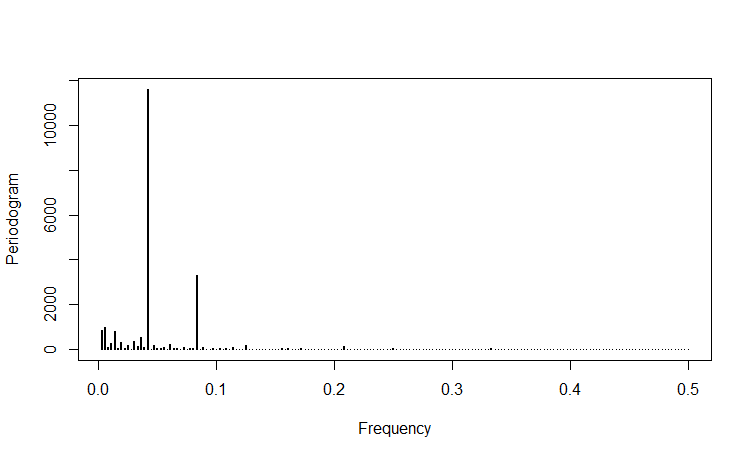
\includegraphics[width=0.8\textwidth]{figures/forecasting/periodogram_July_2014.png}
	\caption{Periodogram of hourly day ahead prices of Nord Pool Spot, Helsinki from July 7th to July 21st in 2014}
	\label{fig:periodogram_July_2014}
\end{figure}

After successfully determine meaningful seasonalities and their resulting periods from the dataset this information can be used to build forecast models that consider the respective seasonal periods in the model generation process. 



\subsection{Seasonal decomposition}

Seasonal decomposition describes the process of decomposing a given time series into its components which are trend, seasonal or cyclic and irregular components. Decomposition is done by applying the STL model to the time series and extracting the above mentioned components where STL is defined as Seasonal-Trend decomposition procedure based on Loess \cite{cleveland1990stl}. 

The decomposition of a time series can be formalized as follows \cite{cleveland1990stl}: 

	\[ Y_v = T_v + S_v + R_v \]
	
where $Y_v$ denotes the original time series, $T_v$ the trend component, $S_v$ the seasonal component and $R_v$ the remainder component. $v \in \{ 1,\ldots,N \}$ denotes an individual time stamp in the series where $N$ is the number of unit time stamps in the time series. 

A sample seasonal decomposition of hourly time series is depicted in Figure \ref{fig:stl_decomposition_July_2014}. 

\begin{figure}[htbp]
	\centering
		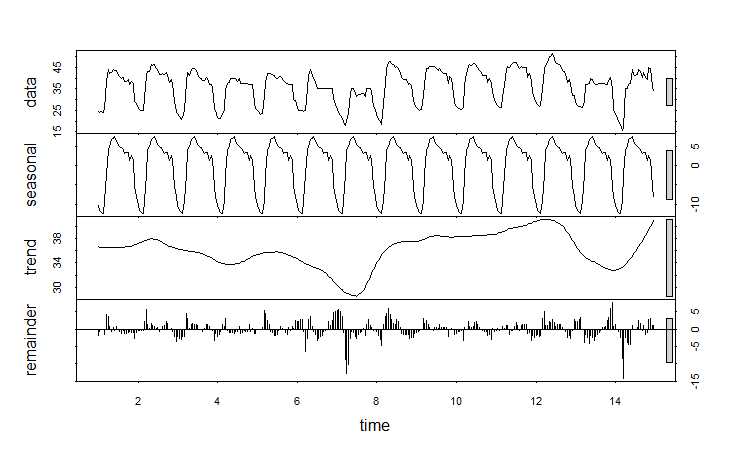
\includegraphics[width=1.00\textwidth]{figures/forecasting/stl_decomposition_July_2014.png}
	\caption{STL decomposition of hourly day ahead time series, Nord Pool Spot, Helsinki from July 7th to July 21st in 2014}	
	\label{fig:stl_decomposition_July_2014}
\end{figure}

The plot consists of four rows with each row containing a different time series component. 
The first row shows the original time series with hourly prices over a time period of two weeks. There are evident daily and weekly seasonal periods visible in the time series. Daily seasonality can be observed by the repetitive pattern of highs and lows over each day whereas weekly seasonality is evident due to the recognizable decline of prices towards the end of each week. 

The second row represents the extracted daily seasonal component which depicts the daily variation in prices. STL is only capable of extracting a single seasonality pattern. In case both daily and weekly seasonal periods should be extracted a BATS or TBATS model can be used (these models are discussed later in this section). 

In the third row the trend component is displayed. It shows a seemingly repetitive pattern over one week, which denotes the weekly seasonal period observable from the original time series. 

Finally in the last row the remaining irregular component is shown which contains all remaining variations in the time series. 

The grey bars at the right hand side of each plot aim to provide a relative comparison of scales over all plots, i.e.~the height of the bars show the same value range in different scales. Thus the whole value range of the trend component is equivalent with the value range of about one third of the original time series. 




\subsection{Forecast models}

Different statistical forecast models have been chosen to be investigated on a large scale. The selection of forecast models includes simpler models such as Simple Exponential Smoothing and more advanced models such as ARIMA and TBATS and variants thereof. The purpose of the evaluation is to provide insights into the performance of different forecast models when applied to electricity price time series. 

\subsubsection{Mean forecast}

The mean forecast is a simple model based on previous observations of a time series. It calculates the mean over a training data set and uses this mean as forecast for all future values \cite{hyndman2012forecasting}. 

It can be formally defined as in equation \ref{eq:mean_forecast}

%\begin{equation}
%\hat{Y}_{t+i} = Y_t
%\label{eq:naive_forecast}
%\end{equation}

\begin{equation}
\hat{y}_{T+h|T} = \frac{1}{T} \sum_{i=1}^T y_i
\label{eq:mean_forecast}
\end{equation}

where $T$ denotes the number of observations in the trainings dataset, $y_i$ denote historical values and $\hat{y}_{T+h|T}$ denotes a forecast of $h$ values into the future beginning at the value of $y_T$. 

Even though the mean forecast only includes simple calculations it can be effective to forecast random or near random time series or time series that exhibit strong volatility. As it is the simplest of the proposed models it should serve as a baseline model to which other models' performance can be compared. 

\subsubsection{Simple Exponential Smoothing}

The Simple Exponential Smoothing model (SES) belongs to the category of exponential smoothing models which calculate the weighted average over historical observations where weights are exponentially decreased for observations in the past. 

As the name implies this model is the simplest of exponential smoothing models which is designed to provide forecast for time series without trend or seasonal components. Similar to the mean forecast model past values of a time series are processed but with given weights that decrease exponentially over time \cite{hyndman2012forecasting,weron2007modeling}. 

The corresponding formula is depicted in Equation \ref{eq:ses_forecast} 

\begin{equation}
\hat{y}_{T+1|T} = \sum_{i=0}^{T-1} \alpha (1 - \alpha)^i y_{T-i}
\label{eq:ses_forecast}
\end{equation}

where $\alpha$ with $0 \le \alpha \le 1$ denotes the smoothing parameter that determines the influence of past observations through setting the corresponding weights. Thus by modifying values of $\alpha$ the resulting impact of past values to forecasted values can be defined. 

\subsubsection{Holt's Exponential Smoothing}

Holt's Exponential Smoothing (Holt's ES) is a linear trend method which extends Simple Exponential Smoothing by including trends in the model generation process \cite{hyndman2012forecasting}. The model consists of two separately modeled components which are level and trend components. These are combined to obtain forecasts for a given time series. It can be formalized by the following equations:

\begin{align}
 \hat{y}_{t+h|t} &= l_t + h b_t \label{eq:holts_forecast} \\
 l_t &= \alpha y_t + (1 - \alpha) (l_{t-1} + b_{t-1})\label{eq:holts_level_component} \\
 b_t &= \beta (l_t - l_{t-1}) + (1 - \beta) b_{t-1}\label{eq:holts_trend_component}
\end{align}

Equation \ref{eq:holts_forecast} denotes the forecast value $\hat{y}_{t+h|t}$ which is forecasted $h$ steps into the future beginning from time stamp $t$. It consists of a combination of the level $l_t$ at time $t$ and the trend $b_t$ at time $t$ continued over the next $h$ time intervals. 

The level component is described in Equation \ref{eq:holts_level_component} which denotes a linear combination of the actual value $y_t$ at time $t$ and the level forecast constructed from previous time stamp's level $l_{t-1}$ and trend $b_{t-1}$ components. 

Equation \ref{eq:holts_trend_component} depicts the trend component which is a linear combination of the difference of the current and previous levels ($l_t, l_{t-1}$) and the estimated trend component $b_{t-1}$ from the previous point in time. 

$\alpha$ and $\beta$ exhibit characteristics $0 \le \alpha \le 1$ and $0 \le \beta \le 1$ and denote the smoothing parameters for the level and trend components, respectively.

\subsubsection{Seasonal HoltWinter's model}

The Seasonal HoltWinter's model is the first of the discussed models which is capable of modeling seasonality in the dataset. It further extends the capabilities of the SES and Holt's ES models by an additional seasonal component. Thus besides the level and trend components $l_t$ and $b_t$ a seasonal component $s_t$ is introduced, with smoothing parameters $\alpha, \beta, \gamma$, respectively \cite{hyndman2012forecasting}. 

The corresponding equations are defined as

\begin{align}
 \hat{y}_{t+h|t} &= l_t + h b_t + s_{t-m+h_m^+} \label{eq:holtwinter_forecast} \\
 l_t &= \alpha (y_t - s_{t-m}) + (1 - \alpha) (l_{t-1} + b_{t-1})\label{eq:holtwinter_forecast_level_component} \\
 b_t &= \beta (l_t - l_{t-1}) + (1 - \beta) b_{t-1}\label{eq:holtwinter_forecast_trend_component} \\
 s_t &= \gamma (y_t - l_{t-1} - b_{t-1}) + (1 - \gamma) s_{t-m}\label{eq:holtwinter_forecast_seasonal_component}
\end{align}

where $m$ denotes the period of seasonality (e.g.~$m=12$ for monthly data when one year is the base unit) and $h_m^+ = \left\lfloor (h-1) \mod m\right\rfloor + 1$ represents the additional number of steps ahead required to model the corresponding seasonal period $m$. Therefore $s_{t-m+h_m^+}$ denotes the previously occurred seasonal period which is added to the forecast equation in Equation \ref{eq:holtwinter_forecast}. 

The level component in Equation \ref{eq:holtwinter_forecast_level_component} is adjusted by the level of the last occurred seasonal period $s_{t-m}$ to consider seasonal differences. The equation for the trend component $b_t$ is taken directly from the one of Holt's ES in Equation \ref{eq:holts_trend_component} whereas the seasonal component is defined in Equation \ref{eq:holtwinter_forecast_seasonal_component}. 

The seasonal component is denoted as a weighted sum of the current value $y_t$ substracted by previous level and trend components and the value of the seasonal component exactly $m$ periods before. 

The smoothing parameters $\alpha, \beta$ and $\gamma$ are estimated by minimizing the squared one-step prediction error to appropriately weigh the different components to yield best results \cite{r2016language}. 


\subsubsection{ARIMA models}

ARIMA models or Auto Regressive Integrated Moving Average models are highly adjustable time series models that can incorporate a number of features from the dataset. They are capable of modeling correlations in the data as well as provide a smoothing method to dampen the impact of extreme outliers. 

ARIMA models may consist of both autoregressive (AR) and moving average (MA) terms to accurately model the underlying dataset \cite{hyndman2012forecasting,weron2007modeling}. 

\paragraph{AR model} The autoregressive component is used to model dependencies in the data such that correlations within the dataset are reduced. It is defined as a weighted sum of past values of an observation. An AR(p) model is shown in Equation \ref{eq:ar_component}.

\begin{equation}
	y_t = c + \sum_{i=1}^p \phi_i y_{t-i} + e_t
\label{eq:ar_component}
\end{equation}

where $y_t$ is modeled as the sum of the past $p$ values of $y$ plus an additional error component $e_t$ and a constant $c$. AR coefficients $\phi_1,\ldots,\phi_p$ are used to weight past observations and need to be estimated in the model generation process. 

\paragraph{MA model} The moving average component models a time series as a moving average of past error terms. Equation \ref{eq:ma_component} gives the formal definition: 

\begin{equation}
	y_t = c + e_t + \sum_{i=1}^q \theta_i e_{t-i}
\label{eq:ma_component}
\end{equation}

where $e_t$ denotes the forecast error at time $t$ and the error terms are weighted by MA coefficients $\theta_1,\ldots,\theta_q$.

\paragraph{ARIMA model} An ARIMA model consist of both AR and MA terms. In addition ARIMA models are able to model non-stationary time series by applying differencing operations to the dataset. ARIMA(p,d,q) denotes a model consisting of $p$ number of AR terms, $q$ MA terms and $d$ number of differences. 
It can be described as the sum of AR and MA terms:

\begin{equation}
	y_t = \sum_{i=1}^p \phi_i y_{t-i} + \sum_{i=1}^q \theta_i e_{t-i} + e_t + c
\label{eq:arima_model}
\end{equation}

When applying the model the possible applied differences during data preprocessing are reversed by integrating the results which refers to the \textit{Integrating} part of the model. 

ARIMA models can be enhanced to model seasonal periods which are defined as ARIMA (p,d,q)(P,D,Q)\textsubscript{m} also denoted as SARIMA models. 
In addition to non-seasonal parameters $p, d$ and $q$ the seasonal parameters $P$, $D$ and $Q$ denote the seasonal AR, differencing and MA components, respectively. 



\subsubsection{BATS and TBATS models}

Multiple seasonal periods can be applied by models such as BATS and TBATS \cite{r2016language}. This can be done by applying a BATS or TBATS model to the time series, identifying different seasonal and trend components and modeling each component separately \cite{de2011forecasting}. 

Both BATS and TBATS models are able to handle multiple seasonalities in the data, i.e.~considering both daily and weekly seasonal periods where TBATS models are capable of modeling non-integer periods as well (e.g.~365.25 for annual seasonality). 

\paragraph{BATS model} BATS stands for Box-Cox transform, ARMA errors, Trend, and Seasonal components. TBATS can then be regarded as the trigonometric version of BATS. 

The definition of BATS is outlined in the following equations: 


\begin{equation}
	y_t^{(\omega)} = 
	\begin{cases}
		\frac{y_t^\omega - 1}{\omega}, & \omega \neq 0 \\
		\log y_t, & \omega = 0
	\end{cases}
\end{equation}


%\begin{equation}
	%y_t^{(\omega)} = 
	%\begin{cases}
		%\frac{y_t^\omega - 1}{\omega}, & \text{if}\ a=1 \\
		%\log y_t, & \text{otherwise}
	%\end{cases}
%\end{equation}


\begin{align}
	y_t^{(\omega)} &= l_{t-1} + \phi b_{t-1} + \sum_{i=1}^T s_{t-m_i}^{(i)} + d_t\label{eq:bats_model} \\
	l_t &= l_{t-1} + \phi b_{t-1} + \alpha d_t \\
	b_t &= (1 - \phi) b + \phi b_{t-1} + \beta d_t \\
	s_t^{(i)} &= s_{t-m_i}^{(i)} + \gamma_i d_t\label{eq:bats_seasonal} \\
	d_t &= \sum_{i=1}^p \Phi_i d_{t-i} + \sum_{i=1}^q \theta_i e_{t-i} + e_t
\end{align}

where $y_t^{(\omega)}$ denotes the Box-Cox transformed value with parameter $\omega$ where $y_t$ is the current value at time $t$. 

$l_t$ describes the level, $b$ denotes the long term trend, $b_t$ represents the trend, $e_t$ is gaussian white noise with zero mean and constant variance and $s_t^{(i)}$ denotes the i-th seasonal component. $\phi$ denotes the damping parameter for the trend and defines the impact of short and long term trends. All of these components are adjusted by a weighted ARMA component $d_t$ and coefficients $\alpha$, $\beta$ and $\gamma$, respectively. 

A BATS model is parameterized by BATS($\omega$,$\phi$,$p$,$q$,$m_1$,\ldots,$m_T$) with the Box-Cox parameter $\omega$, damping parameter $\phi$, ARMA parameters $p$ and $q$ and seasonal periods $m_1,\ldots,m_T$. A double seasonal model (e.g.~daily and weekly) with an AR(1) component can be described as BATS(1,1,1,0,$m_1$,$m_2$) with default Box-Cox and damping parameters. 

\paragraph{TBATS model} As BATS models possibly result in a large number of states and only pure integer seasonal periods may be modeled, the TBATS model has been developed \cite{de2011forecasting}. This model enhances the BATS model with trigonometric expressions:

%It is formalized as follows: 

\begin{align}
	s_t^{(i)} &= \sum_{j=1}^{k_i} s_{j,t}^{(i)}\label{eq:tbats_seasonal} \\
	s_{j,t}^{(i)} &= s_{j,t-1}^{(i)} \cos \lambda_j^{(i)} + s_{j,t-1}^{*(i)} \sin \lambda_j^{(i)} + \gamma_1^{(i)} d_t \\
	s_{j,t}^{*(i)} &= - s_{j,t-1} \sin \lambda_j^{(i)} + s_{j,t-1}^{*(i)} \cos \lambda_j^{(i)} + \gamma_2^{(i)} d_t 
\end{align}

where $s_{j,t}^{(i)}$ describes the stochastic level of the i-th seasonal component and $s_{j,t}^{*(i)}$ represents the stochastic growth in the level of the i-th seasonal component which can be described as the change of value of the seasonal component over a period of time. $k_i$ is the number of harmonics required for the ith seasonal component, $\gamma_1^{(i)}$ and $\gamma_2^{(i)}$ are smoothing parameters and $\lambda_j^{(i)} = \frac{2 \pi j}{m_i}$ the trigonometric parameter which depends on the corresponding seasonal period $m_i$. 

Finally the model can be obtained by replacing $s_t^{(i)}$ in equation \ref{eq:bats_seasonal} by the trigonometric expression in equation \ref{eq:tbats_seasonal} and replacing $s_{t-m_i}^{(i)}$ in equation \ref{eq:bats_model} by $s_{t-1}^{(i)}$. 

%\begin{equation}
	%y_t^{(\omega)} = l_{t-1} + \phi b_{t-1} + \sum_{i=1}^T s_{t-1}^{(i)} + d_t
%\label{eq:tbats_model}
%\end{equation}

\section{Model generation}





\section{Model selection algorithm}



\section{R / Java Simulation Framework}



\section{Forecast model evaluation}





%  Generated from R function getRMSEResults: Get results from forecast simulation 
% -----------------------
% Get results from forecast simulation for the given location
% over a time range of 3 years, generate models in intervals of 1 week
% with 2,3 and 4 weeks of trainings data periods
% 5 locations are available from the forecast simulation (Application server):
%  1) Hamina, locationId 1, DA
%  2) St.Ghislain, locationId 2, DA
%  3) Portland, locationId 4, RT
%  4) Richmond, locationId 6, RT
%  5) Hatfield, locationId 8, RT






%%%  General results - all numbers  %%%


Four simulations have been run for four different locations over three years of energy price data. 
For each of these locations three different training periods have been evaluated: two weeks, three weeks and four weeks. 
Each of these simulations is evaluated for five different accuracy measures: 

\begin{itemize}
	\item Mean error (ME)
	\item Mean absolute error (MAE)
	\item Root mean squared error (RMSE)
	\item Mean percentage error (MPE)
	\item Mean absolute percentage error (MAPE)
\end{itemize}

In addition, each of these error measures has been evaluated for ten different forecast horizons (in hours): 
1, 3, 6, 12, 18, 24, 36, 48, 96, 168. 

In the tables below results are shown aggregated by forecast horizon for each accuracy measure. Each table depicts a different training period for the given location. 



\subsection{Forecast evaluation results}

% latex table generated in R 3.1.1 by xtable 1.8-2 package
% Mon Mar 07 23:15:14 2016
\begin{table}[ht]
\centering
\begin{tabular}{rrrrrrr}
  \hline
 & mean & ses & holts & holtwinters & arima & tbats \\ 
  \hline
2 weeks & 14.55 & 11.60 & 62.76 & 73.65 & 10.23 & 8.19 \\ 
  3 weeks & 14.78 & 11.60 & 62.90 & 74.02 & 9.53 & 8.59 \\ 
  4 weeks & 14.99 & 11.60 & 63.23 & 85.06 & 9.26 & 8.44 \\ 
   \hline
\end{tabular}
\caption{Results of evaluation for Hamina, Nord Pool Spot (DA)} 
\end{table}


% latex table generated in R 3.1.1 by xtable 1.8-2 package
% Mon Mar 07 23:15:14 2016
\begin{table}[ht]
\centering
\begin{tabular}{rrrrrrr}
  \hline
 & mean & ses & holts & holtwinters & arima & tbats \\ 
  \hline
2 weeks & 17.07 & 15.23 & 127.13 & 186.82 & 13.49 & 1.27E+50 \\ 
  3 weeks & 17.40 & 15.27 & 128.05 & 190.21 & 12.94 & 11.60 \\ 
  4 weeks & 17.59 & 15.30 & 127.03 & 186.37 & 12.87 & 2.49E+36 \\ 
   \hline
\end{tabular}
\caption{Results of evaluation for St.Ghislain, Belpex (DA)}
\end{table}
% latex table generated in R 3.1.1 by xtable 1.8-2 package
% Mon Mar 07 23:15:14 2016
\begin{table}[ht]
\centering
\begin{tabular}{rrrrrrr}
  \hline
 & mean & ses & holts & holtwinters & arima & tbats \\ 
  \hline
2 weeks & 24.22 & 23.61 & 235.84 & 407.06 & 24.03 & 5.45E+16 \\ 
  3 weeks & 24.14 & 23.56 & 238.92 & 686.95 & 22.26 & 1.64E+18 \\ 
  4 weeks & 24.68 & 23.32 & 268.10 & 437.85 & 21.91 & 2.18E+32 \\ 
   \hline
\end{tabular}
\caption{Results of evaluation for Portland, ISO-NE (RT)}
\end{table}
% latex table generated in R 3.1.1 by xtable 1.8-2 package
% Mon Mar 07 23:15:14 2016
\begin{table}[ht]
\centering
\begin{tabular}{rrrrrrr}
  \hline
 & mean & ses & holts & holtwinters & arima & tbats \\ 
  \hline
2 weeks & 14.47 & 15.17 & 148.54 & 322.41 & 15.03 & 7.57E+13 \\ 
  3 weeks & 14.46 & 15.23 & 147.77 & 318.61 & 14.14 & 13.46 \\ 
  4 weeks & 14.42 & 15.29 & 148.67 & 357.82 & 14.11 & 5.44E+108 \\ 
   \hline
\end{tabular}
\caption{Results of evaluation for Richmond, PJM (RT)}
\end{table}



